\documentclass[preview]{standalone}
\usepackage[siunitx, american]{circuitikz}
% SOLUCIÓN 1: Cargar explícitamente arrows.meta para que funcione Triangle[fill=black]
\usetikzlibrary{positioning, arrows.meta}

\tikzset{
	% 1. Válvula Forrester con máscara de fondo (=== X ===)
	pics/sdvalve/.style={
		code={
			\fill[white] (-0.3, -0.25) rectangle (0.3, 0.25);
			\draw[thick, fill=white] (-0.25, 0.2) -- (0,0) -- (-0.25, -0.2) -- cycle;
			\draw[thick, fill=white] (0.25, 0.2) -- (0,0) -- (0.25, -0.2) -- cycle;
			\draw[thick] (-0.25, 0.2) -- (-0.25, -0.2);
			\draw[thick] (0.25, 0.2) -- (0.25, -0.2);
		}
	},
	% 2. Nube clásica de Forrester
	pics/sdcloud/.style={
		code={
			% Curva con valles elevados a altura y=0.8
			\draw[xscale=0.10, yscale=0.18,semithick, fill=blue!0]
			(-3, 0) .. controls (-4, 1.2) and (-1.8, 1.2) .. (-1.4, 0.8)
			.. controls (-0.9, 1.8) and (0.9, 1.8) .. (1.4, 0.8)
			.. controls (1.8, 1.2) and (4, 1.2) .. (3, 0);
			% Repetición
			\draw[xscale=0.10, yscale=0.18, semithick, fill=blue!0]
			(-3, 0) .. controls (-4, -1.2) and (-1.8, -1.2) .. (-1.4, -0.8)
			.. controls (-0.9, -1.8) and (0.9, -1.8) .. (1.4, -0.8)
			.. controls (1.8, -1.2) and (4, -1.2) .. (3, 0);
		}
	},
	% 3. Icono de Parámetro nativo de AnyLogic
	pics/alparam/.style={
		code={
			\draw[thick, fill=white] (0,0) circle (0.19);
			\draw[fill] (-0.01, 0.02) -- (-0.12, 0.25) -- (-0.23, 0.15) -- cycle;
		}
	},
	pics/alparal/.style={
		code={
			\draw[thick, fill=white] (0,0) circle (0.19);
			\draw[fill] (0.01, 0.02) -- (0.12, 0.25) -- (0.23, 0.15) -- cycle;
		}
	}
}


\begin{document}
\begin{figure}[htbp]
    \centering
    \resizebox{\textwidth}{!}{%
      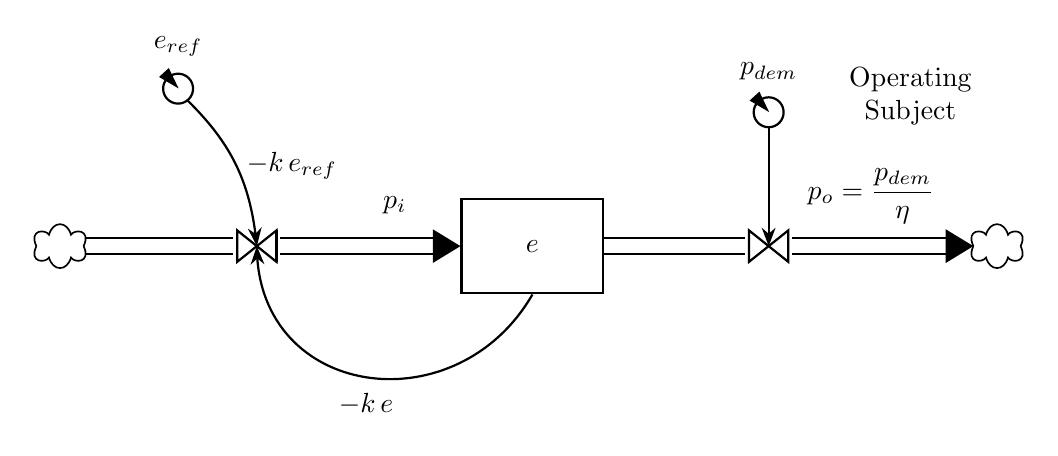
\begin{tikzpicture}[
        stock/.style={rectangle, draw=black, thick, minimum width=1.8cm, minimum height=1.2cm, fill=white, align=center},
        flow/.style={
          draw=black,
          thick,
          double,
          double distance=5pt,
          fill=white
        },
        flow_arrow/.style={
          flow,
          -{Triangle[fill=black, length=10pt, width=12pt]}
        },
        sdarrow/.style={-Stealth, thick, color=black, >=Stealth}
        ]
        % --- 1. STOCK CENTRAL ---
        \node[stock] (e) at (0,0) {$e$};
        % --- 2. COORDENADAS DE FRONTERA Y VÁLVULAS ---
        \coordinate (c_in) at (-6, 0);
        \coordinate (v_in) at (-3.5, 0);

        \coordinate (v_out) at (3, 0);
        \coordinate (c_out) at (6, 0);
        % --- 3. PARÁMETROS ESTILO ANYLOGIC ---
        \coordinate (eref) at (-4.5, 2.0);
        \pic at (eref) {alparam};
        \node[above=8pt, scale=1.0] at (eref) {$e_{ref}$};
        \coordinate (pd) at (3, 1.7);
        \pic at (pd) {alparam};
        \node[above=8pt, scale=1.0] at (pd) {$p_{dem}$};
        \node[text width=1.8cm, align=center,xshift=18mm,yshift=2mm] at (pd) {Operating Subject};
        % --- 4. DIBUJO DE FLUJOS ---
        % Flujo de Inyección (p_i)
        \draw[flow] (c_in) -- (v_in);
        % SOLUCIÓN 2: Detener la línea en el borde (e.west) para que se vea la punta de entrada
        \draw[flow_arrow] (v_in) -- (e.west);
        \node[above=8pt, scale=1.0] at (-1.75, 0) {$p_i$};
        % Flujo de Consumo (p_o)
        % SOLUCIÓN 3: Salir desde el borde (e.east) de forma limpia
        \draw[flow] (e.east) -- (v_out);
        % SOLUCIÓN 4: Ajustar destino a (5.7, 0) para frenar justo al tocar la nube
        \draw[flow_arrow] (v_out) -- node[midway, above=1ex]
        {$\displaystyle p_o = \frac{p_{dem}}{\eta}$} ++(2.6, 0);
        %\node[above=8pt, scale=1.0] at (1.75, 0) {$p_o$};
        % --- 5. DIBUJO DE COMPONENTES OPACOS (Válvulas y Nubes) ---
        \pic at (v_in) {sdvalve};
        \pic at (v_out) {sdvalve};
        \pic at (c_in) {sdcloud};
        \pic[xshift=-1mm] at (c_out) {sdcloud};
        % --- 6. LAZOS DE INFORMACIÓN DIRIGIDOS ---
        \draw[sdarrow] (eref)+(.11,-.14) to[bend left=20] node[midway, right] {$-k\, e_{ref}$} (v_in);
        \draw[sdarrow] (e.south) to[out=-120, in=-90, looseness=1.4] node[midway, below=2pt] {$-k\, e$} (v_in);
        \draw[sdarrow] (pd)+(0,-.18) --  (v_out);
      \end{tikzpicture}%
    }
 \end{figure}

\end{document}
